\documentclass[11pt,letterpaper]{article}

\usepackage[margin=1in]{geometry}
\usepackage[T1]{fontenc}
\usepackage{newtxtext,newtxmath}
\usepackage{microtype}
\usepackage{amsmath}
\usepackage{graphicx}
\usepackage{booktabs}
\usepackage[font=small,labelfont=bf,skip=4pt]{caption}
\usepackage[compact,small]{titlesec}
\usepackage{enumitem}
\setlist{itemsep=2pt,topsep=3pt,parsep=0pt,leftmargin=*}
\usepackage[dvipsnames]{xcolor}
\usepackage[colorlinks=true,linkcolor=MidnightBlue,citecolor=MidnightBlue,urlcolor=MidnightBlue]{hyperref}

\graphicspath{{figures/}}
% Let floats share pages with text instead of collecting on sparse float pages.
\renewcommand{\topfraction}{0.9}
\renewcommand{\bottomfraction}{0.9}
\renewcommand{\textfraction}{0.05}
\renewcommand{\floatpagefraction}{0.9}
\setcounter{topnumber}{4}
\setcounter{bottomnumber}{4}
\setcounter{totalnumber}{6}
\setlength{\textfloatsep}{10pt plus 2pt minus 4pt}
\setlength{\floatsep}{10pt plus 2pt minus 2pt}
\setlength{\parindent}{0pt}
\setlength{\parskip}{3pt}
\newcommand{\tablefont}{\footnotesize\setlength{\tabcolsep}{3.4pt}}

\title{\vspace{-1.5em}\textbf{Do Stocks Outperform Treasury Bills?}\\[2pt]
  \large Simulated Multi-Period Returns and Industry Portfolios, after Bessembinder (2018)}
\author{Yingni Chang, Yikai Shen}
\date{September 2026}

\begin{document}
\maketitle
\vspace{-1.5em}

\section*{Summary}

We replicate Bessembinder's Table 1 and extend it to daily returns and longer horizons. The assigned daily
mean is much lower than the paper's monthly mean, so median returns become negative even at moderate
volatility. At 20 years and 20\% monthly volatility, the median return is $-97.9\%$, although the expected
return remains $+231\%$. Compounding can explain this gap between typical and average outcomes, but it
does not by itself explain the low-volatility anomaly in arithmetic returns or alphas.

For Table 4, we replace random stocks with industry portfolios. Equal-weighted FF49 industries beat the
market more often than value-weighted industries. Selecting the best industry over the previous three
months produces a high terminal return with EW stocks, but also a 99.7\% drawdown. Holding the five best
industries over the previous six months gives stronger historical ten-year win rates. These results are
before costs, and overlapping historical windows do not establish a future outperformance probability.

%======================================================================================================
\section{Simulated multi-period returns (Table 1)}

\subsection{Simulation method}

Returns are i.i.d.\ $r_t \sim N(\mu, \sigma^2)$, and the $T$-period buy-and-hold return is
$\prod_{t=1}^{T}(1+r_t) - 1$. Each experiment simulates 250,000 paths. The 1- and 5-year outcomes come from
non-overlapping blocks of the 10-year paths, and the 15- and 20-year outcomes from 240-month paths. We report one
set of draws (seed~0); four further independent runs (seeds 1--4) measure Monte Carlo error. Simulated means and
SDs are z-tested against exact values from $E[W_T^k]$, where $W_T = \prod_t (1+r_t)$ (e.g.\ $E[W_T] = (1+\mu)^T$).
We apply the z-tests where exact skewness is below 10; heavier tails make the normal approximation unreliable.
All applicable tests pass.
Draws below $-100\%$ are kept. Treating them as an absorbing bankruptcy changes no median, share or percentile. Our
monthly replication matches Table~1 to within 0.35 points on the median and 0.18 points on the share positive
(Table~\ref{tab:compare}).

\subsection{Daily returns}

We draw 2,520 daily returns (252 a year) with $\mu = 0.0025\%$ and daily $\sigma = 0.45\%, 0.90\%, \dots, 4.5\%$.
We pair these with the paper's monthly columns $2\%, \dots, 20\%$, since $0.45\% \times \sqrt{21} \approx 2\%$.
Table~\ref{tab:daily} gives the result in the layout of Table~1.

\begin{table}[!htbp]
  \centering\tablefont
  \caption{Table~1 with \textbf{daily} normal returns, $\mu = 0.0025\%$ a day (seed 0, 250,000 paths).}
  \label{tab:daily}
  \begin{tabular}{@{}llrrrrrrrrrrr@{}}
\toprule
 & & \multicolumn{11}{c}{Daily $\sigma$ (\%)} \\ \cmidrule(l){3-13}
Statistic & Horizon & 0.00 & 0.45 & 0.90 & 1.35 & 1.80 & 2.25 & 2.70 & 3.15 & 3.60 & 4.05 & 4.50 \\
& & \multicolumn{11}{c}{\textit{paired monthly column in the paper (\%)}} \\
& & 0 & 2 & 4 & 6 & 8 & 10 & 12 & 14 & 16 & 18 & 20 \\ \midrule
Skewness & 1y & -- & 0.22 & 0.43 & 0.66 & 0.90 & 1.15 & 1.43 & 1.74 & 2.08 & 2.48 & 2.94 \\
 & 5y & -- & 0.49 & 1.02 & 1.65 & 2.47 & 3.63 & 5.37 & 8.18 & 12.9 & 20.8 & 34.0 \\
 & 10y & -- & 0.69 & 1.51 & 2.63 & 4.35 & 7.21 & 12.1 & 20.1 & 32.4 & 49.3 & 70.0 \\
\addlinespace
Median (\%) & 1y & 0.6 & 0.4 & $-$0.4 & $-$1.6 & $-$3.4 & $-$5.6 & $-$8.2 & $-$11.2 & $-$14.5 & $-$18.1 & $-$22.0 \\
 & 5y & 3.2 & 1.9 & $-$1.9 & $-$7.9 & $-$15.8 & $-$24.9 & $-$34.7 & $-$44.7 & $-$54.3 & $-$63.3 & $-$71.2 \\
 & 10y & 6.5 & 3.9 & $-$3.7 & $-$15.2 & $-$29.0 & $-$43.6 & $-$57.4 & $-$69.4 & $-$79.1 & $-$86.5 & $-$91.7 \\
\addlinespace
\% $>0$ & 1y & 100.0 & 52.1 & 48.9 & 46.9 & 45.2 & 43.6 & 42.1 & 40.7 & 39.2 & 37.8 & 36.4 \\
 & 5y & 100.0 & 54.7 & 47.6 & 43.2 & 39.4 & 36.0 & 32.8 & 29.8 & 27.0 & 24.3 & 21.8 \\
 & 10y & 100.0 & 56.8 & 46.7 & 40.4 & 35.2 & 30.6 & 26.5 & 22.7 & 19.2 & 16.2 & 13.5 \\
\addlinespace
99th pct.\ (\%) & 1y & 0.6 & 18.5 & 38.9 & 61.9 & 87.7 & 116.6 & 148.7 & 184.0 & 222.8 & 265.0 & 310.6 \\
 & 5y & 3.2 & 47.8 & 106.5 & 180.9 & 272.8 & 382.3 & 508.0 & 647.4 & 795.7 & 947.2 & 1,093 \\
 & 10y & 6.5 & 75.8 & 175.7 & 311.1 & 482.5 & 684.8 & 905.4 & 1,124 & 1,315 & 1,452 & 1,523 \\
\bottomrule
\end{tabular}

\end{table}

\begin{table}[!htbp]
  \centering\tablefont
  \caption{Comparison with Table~1 at the 10-year horizon. ``Matched $\mu$'' is $1.005^{1/21} - 1 = 0.0238\%$ a
    day, i.e.\ the paper's 0.5\% a month.}
  \label{tab:compare}
  \begin{tabular}{@{}llrrrrrrrrrrr@{}}
\toprule
& Monthly $\sigma$ (\%) & 0 & 2 & 4 & 6 & 8 & 10 & 12 & 14 & 16 & 18 & 20 \\
& Daily $\sigma$ (\%) & 0.00 & 0.45 & 0.90 & 1.35 & 1.80 & 2.25 & 2.70 & 3.15 & 3.60 & 4.05 & 4.50 \\ \midrule
Median (\%) & Paper, monthly & 81.9 & 77.7 & 65.6 & 47.3 & 24.3 & 0.1 & $-$23.5 & $-$44.6 & $-$62.0 & $-$75.7 & $-$85.3 \\
 & Ours, monthly & 81.9 & 77.7 & 65.5 & 47.0 & 24.4 & 0.1 & $-$23.5 & $-$44.6 & $-$62.0 & $-$75.5 & $-$85.2 \\
 & Ours, daily, $\mu = 0.0025\%$ & 6.5 & 3.9 & $-$3.7 & $-$15.2 & $-$29.0 & $-$43.6 & $-$57.4 & $-$69.4 & $-$79.1 & $-$86.5 & $-$91.7 \\
 & Ours, daily, matched $\mu$ & 81.9 & 77.5 & 64.5 & 44.9 & 21.3 & $-$3.5 & $-$27.1 & $-$47.7 & $-$64.3 & $-$76.9 & $-$85.8 \\
\addlinespace
\% $>0$ & Paper, monthly & 100.0 & 99.6 & 87.5 & 72.1 & 59.7 & 50.0 & 42.1 & 35.2 & 29.5 & 24.2 & 20.0 \\
 & Ours, monthly & 100.0 & 99.6 & 87.6 & 72.2 & 59.9 & 50.1 & 42.1 & 35.2 & 29.4 & 24.3 & 20.0 \\
 & Ours, daily, $\mu = 0.0025\%$ & 100.0 & 56.8 & 46.7 & 40.4 & 35.2 & 30.6 & 26.5 & 22.7 & 19.2 & 16.2 & 13.5 \\
 & Ours, daily, matched $\mu$ & 100.0 & 99.4 & 86.5 & 70.8 & 58.5 & 48.7 & 40.8 & 34.1 & 28.4 & 23.5 & 19.3 \\
\bottomrule
\end{tabular}

\end{table}

The assigned daily mean compounds to only $0.0525\%$ over 21 days, about a tenth of
    the paper's 0.5\% a month. This leaves little expected growth to offset volatility drag. The median is negative and fewer than half of
    outcomes are positive from daily $\sigma = 0.90\%$ (monthly $\approx 4\%$) at all horizons. In the paper, this
    happens only from 12\% monthly. As a rough guide, the small-return approximation to typical log growth,
    $\mu - \sigma^2/2$, turns negative near $\sigma \approx 0.71\%$ daily.

With the matched mean, the daily table is close
    to Table~1: medians are at most 3.7 points below the paper's. The larger part of the gap is the grid. The daily
    $\sigma$ values correspond to monthly 2.07\%--20.9\%, not 2\%--20\%, which lowers the median by up to 5.4 points
    (five-seed mean). Drawing daily rather than monthly moves the median by at most 0.6 points at 1 year and 2.8
    points at 10 years.

Right skewness grows with $\sigma$ and horizon, as in Table~1. At long horizons and high
    $\sigma$, this sample size cannot recover it: with $n = 250{,}000$ ten-year outcomes, sample skewness cannot
    exceed $(n-2)/\sqrt{n-1} \approx 500$. At 10 years and 20\% monthly, the exact value is 662, the paper reports
    53.3, and our seeds give 46--186.


\subsection{Horizons of 15 and 20 years}

We use the paper's monthly parameters, $\mu = 0.5\%$ and $\sigma = 0\%, 2\%, \dots, 20\%$ (Table~\ref{tab:long},
Figure~\ref{fig:table1}).

\begin{table}[!htbp]
  \centering\tablefont
  \caption{Table~1 extended to \textbf{15 and 20 years}: monthly normal returns, $\mu = 0.5\%$ (seed 0,
    250,000 paths). ``Exact'' rows are population values from $E[W_T^k]$.}
  \label{tab:long}
  \begin{tabular}{@{}llrrrrrrrrrrr@{}}
\toprule
 & & \multicolumn{11}{c}{Monthly $\sigma$ (\%)} \\ \cmidrule(l){3-13}
Statistic & Horizon & 0 & 2 & 4 & 6 & 8 & 10 & 12 & 14 & 16 & 18 & 20 \\ \midrule
Skewness, sample & 15y & -- & 0.83 & 1.87 & 3.55 & 6.77 & 13.5 & 27.0 & 49.6 & 80.2 & 115 & 149 \\
 & 20y & -- & 0.97 & 2.28 & 4.56 & 9.04 & 17.8 & 33.3 & 56.6 & 86.5 & 121 & 158 \\
\addlinespace
Skewness, exact & 15y & -- & 0.83 & 1.89 & 3.64 & 7.24 & 16.5 & 45.6 & 155 & 632 & 3,037 & 16,689 \\
 & 20y & -- & 0.97 & 2.34 & 4.98 & 12.0 & 36.6 & 149 & 793 & 5,331 & 43,718 & 425,770 \\
\addlinespace
Median (\%) & 15y & 145.4 & 136.9 & 112.9 & 78.0 & 38.3 & $-$0.2 & $-$33.4 & $-$59.1 & $-$76.9 & $-$88.1 & $-$94.4 \\
 & 20y & 231.0 & 215.8 & 174.0 & 116.1 & 54.4 & $-$0.1 & $-$41.9 & $-$69.6 & $-$85.8 & $-$94.2 & $-$97.9 \\
\addlinespace
\% $>0$ & 15y & 100.0 & 99.9 & 92.1 & 76.3 & 61.8 & 49.9 & 40.2 & 32.0 & 25.3 & 19.7 & 15.1 \\
 & 20y & 100.0 & 100.0 & 94.9 & 79.5 & 63.6 & 50.0 & 38.7 & 29.6 & 22.2 & 16.4 & 11.7 \\
\addlinespace
99th pct.\ (\%) & 15y & 145.4 & 340.2 & 635.1 & 1,045 & 1,560 & 2,145 & 2,742 & 3,245 & 3,540 & 3,619 & 3,398 \\
 & 20y & 231.0 & 546.0 & 1,046 & 1,750 & 2,629 & 3,562 & 4,372 & 4,855 & 4,887 & 4,442 & 3,613 \\
\addlinespace
Mean, exact (\%) & 20y & 231.0 & 231.0 & 231.0 & 231.0 & 231.0 & 231.0 & 231.0 & 231.0 & 231.0 & 231.0 & 231.0 \\
\bottomrule
\end{tabular}

\end{table}

\begin{figure}[!htbp]
  \centering
  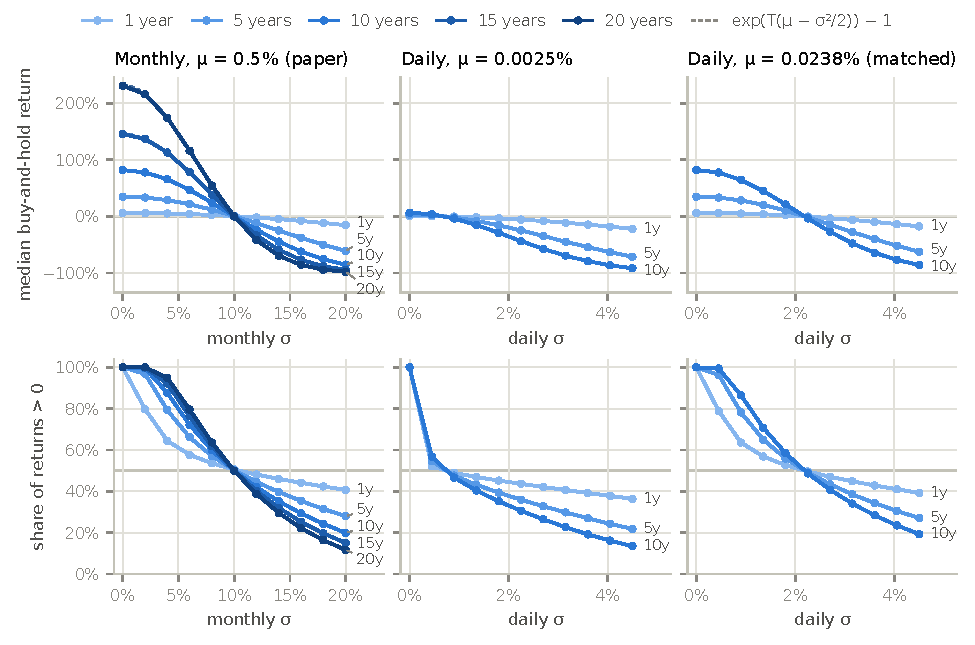
\includegraphics[width=\textwidth]{fig_table1.pdf}
  \caption{Median buy-and-hold return (top) and share of positive outcomes (bottom) against volatility, by
    horizon (seed 0). Dashed lines show the lognormal approximation of the median, $e^{T(\mu - \sigma^2/2)} - 1$.}
  \label{fig:table1}
\end{figure}

The expected 20-year return is 231\% at every
    $\sigma$. The median rises with horizon for $\sigma \le 8\%$ and falls for $\sigma \ge 12\%$. At 10\% it stays
    near zero, and its sign varies across seeds. At 20\% it is $-97.9\%$ after 20 years, with only 11.7\% of
    outcomes positive.

The 99th percentile rises with horizon at every $\sigma$. Over
    20 years it peaks at $\sigma = 16\%$ (4,887\%). The exact skewness at 20\% is 425,770, but the sample value is
    158. Even with 250,000 paths, the seeds' sample means (192.8\%--221.9\%) fall short of the true 231\%, because
    the mass sits in paths too rare to sample.


\subsection{Comparison with Table 1}

The daily and longer-horizon simulations follow the same pattern as Table 1. At a given expected
return, higher volatility means a lower median, a lower chance of a gain and a longer right tail, and each effect
grows with horizon. This is the mechanism behind the paper's finding that most stocks underperform T-bills while a
few account for the aggregate gains.

\subsection{Implications for the low-volatility puzzle}

Compounding lowers the typical terminal wealth of volatile assets at equal expected returns, but it does not explain
the empirical anomaly, which concerns arithmetic average returns and alphas.
At the same expected 10-year return of 81.9\%, the median outcome is
    $+65.5\%$ at $\sigma = 4\%$ but $-62.0\%$ at $\sigma = 16\%$, and the probability of a gain falls from 87.6\% to
    29.4\%. Higher volatility thus lowers typical terminal wealth and the chance of a gain with no difference in
    expected returns. As a small-return approximation, it lowers typical log growth by about $\sigma^2/2$ per period
    (under the literal normal model, returns below $-100\%$ have positive probability, so $E[\log(1+r)]$ is not
    defined). These are comparisons of marginal distributions; we do not estimate how often a high-volatility asset
    trails a low-volatility one.

The anomaly (Ang et al.\ 2006; Baker, Bradley and Wurgler 2011; Frazzini
    and Pedersen 2014) is that high-volatility or high-beta stocks earn lower \emph{average} returns and negative
    alphas. The simulation holds the arithmetic mean fixed by construction, so it cannot produce that.

Compounding makes high-volatility stocks strongly right-skewed, like lotteries.
    If investors prefer positive skewness, they overpay for such stocks and lower their expected returns. This is
    consistent with Table~1 but not tested here. The simulation uses total volatility,
    whereas the literature sorts on idiosyncratic volatility or beta; and cumulative-wealth comparisons alone cannot
    identify differences in expected returns.


%======================================================================================================
\section{Industry portfolios (Table 4)}

\subsection{Data}

We use Ken French's 49 (main) and 12 (robustness) industry portfolios, with monthly equal-weighted (EW) and
value-weighted (VW) returns, from the August 2026 CRSP release. The VW market return is Mkt$-$RF $+$ RF, and the
T-bill return is RF. The sample is the paper's, July 1926 to December 2016 (1,086 months). French assigns stocks to
industries each June but does not date his firm counts, so we assume that a positive July firm count means the
industry had members at the preceding June formation, and treat it as eligible for that July--June year. This gives
40 FF49 industries in 1926 and all 49 from 1969; FF12 always has 12. The universe is thus reconstructed from revised
data; it does not show what an investor could have known at the time.

\subsection{Evaluation method}

The evaluation follows the paper. The horizons are the 90 calendar years 1927--2016, the paper's nine decades (the
first running from July 1926 to December 1936) and the full period. A strategy ``beats'' a benchmark when its
holding-period wealth is strictly higher over the same window. For random strategies, statistics are pooled over
all path $\times$ window outcomes. The paper does not document how it pools windows, so this is our choice. For a
deterministic strategy they are frequencies across historical windows. Monte Carlo standard errors of the pooled
shares are at most 0.35 points.

\subsection{Random industry selection}\label{sec:random}

Each month we draw one eligible industry uniformly at random, hold it for the month, then draw again. We run
20,000 paths with seed 0. The same draws are applied to EW and VW returns, so the two differ only in how stocks are
weighted within the industry. Conditional on history, the expected wealth of this strategy is exact:
\begin{equation}
  E[W] = \prod_t \frac{1}{|A_t|}\sum_{i \in A_t} (1 + r_{i,t}),
  \label{eq:exact}
\end{equation}
where $A_t$ is the eligible set. This is the wealth of an equal-weight portfolio of industries, rebalanced monthly.
Every formally tested simulated mean passes a z-test against it (a normal approximation at a nominal 0.1\%
Bonferroni family-wise level per variant, with a minimum threshold of 4). The heavy-tailed FF49 full-period rows are
reported as diagnostics only.

\begin{table}[!htbp]
  \centering\tablefont
  \caption{Table~4 with \textbf{random industries} in place of random stocks (20,000 paths, July 1926 to December
    2016). ``Ours'' is pooled across paths and windows. The paper's columns are its 1-, 5-, 25-, 50- and 100-stock
    portfolios. Full-period mean and median are in whole percent. Skewness values are Monte Carlo estimates; the
    FF49 full-period values are especially sensitive to rare paths (exact values 80.3 EW and 78.6 VW).}
  \label{tab:table4}
  \begin{tabular}{@{}llrrrrrrrrr@{}}
\toprule
& & \multicolumn{4}{c}{Random industry (ours)} & \multicolumn{5}{c}{Random stocks (paper)} \\
\cmidrule(lr){3-6} \cmidrule(l){7-11}
Horizon & Statistic & FF49 EW & FF49 VW & FF12 EW & FF12 VW & 1 & 5 & 25 & 50 & 100 \\ \midrule
1 year & Mean (\%) & 17.11 & 13.25 & 16.76 & 12.53 & 16.56 & 13.16 & 12.26 & 12.08 & 11.95 \\
 & Median (\%) & 13.99 & 12.26 & 16.04 & 13.17 & 4.06 & 10.72 & 12.52 & 12.90 & 13.18 \\
 & Skewness & 1.75 & 1.32 & 0.49 & 0.06 & 6.99 & 1.08 & 0.10 & $-$0.09 & $-$0.21 \\
 & \% $>0$ & 67.75 & 68.67 & 69.38 & 72.36 & 53.59 & 64.33 & 70.00 & 71.21 & 72.00 \\
 & \% $>$ T-bill & 63.59 & 63.64 & 65.68 & 66.76 & 50.79 & 59.98 & 64.94 & 66.19 & 67.09 \\
 & \% $>$ VW market & \textbf{51.69} & \textbf{48.97} & \textbf{54.47} & \textbf{50.42} & \textbf{42.86} & \textbf{47.20} & \textbf{48.69} & \textbf{49.10} & \textbf{49.28} \\
\midrule
10 years & Mean (\%) & 268.59 & 196.98 & 262.29 & 191.73 & 245.38 & 191.80 & 181.88 & 179.80 & 178.05 \\
 & Median (\%) & 203.40 & 160.05 & 227.28 & 166.81 & 27.72 & 123.64 & 139.77 & 140.09 & 137.60 \\
 & Skewness & 3.71 & 2.77 & 1.56 & 0.99 & 65.03 & 9.03 & 1.64 & 1.15 & 0.90 \\
 & \% $>0$ & 95.77 & 90.97 & 99.32 & 98.16 & 56.18 & 83.60 & 95.96 & 98.38 & 99.57 \\
 & \% $>$ T-bill & 90.34 & 82.57 & 97.72 & 91.80 & 47.77 & 72.29 & 86.86 & 90.70 & 93.08 \\
 & \% $>$ VW market & \textbf{59.54} & \textbf{46.39} & \textbf{69.50} & \textbf{51.81} & \textbf{29.38} & \textbf{40.77} & \textbf{45.37} & \textbf{46.70} & \textbf{47.54} \\
\midrule
Full period & Mean (\%) & 7,573,243 & 1,173,532 & 6,854,963 & 994,527 & 949,826 & 895,497 & 635,547 & 586,071 & 544,181 \\
 & Median (\%) & 2,051,121 & 317,262 & 4,041,583 & 596,943 & 9.5 & 94,936 & 317,456 & 384,332 & 421,749 \\
 & Skewness & 23.32 & 15.82 & 5.75 & 4.91 & 96.45 & 47.24 & 10.02 & 4.40 & 2.95 \\
 & \% $>0$ & 100.00 & 100.00 & 100.00 & 100.00 & 50.76 & 99.94 & 100.00 & 100.00 & 100.00 \\
 & \% $>$ T-bill & 100.00 & 99.89 & 100.00 & 100.00 & 27.45 & 96.48 & 100.00 & 100.00 & 100.00 \\
 & \% $>$ VW market & \textbf{81.23} & \textbf{39.22} & \textbf{97.97} & \textbf{56.75} & \textbf{3.97} & \textbf{22.68} & \textbf{36.81} & \textbf{40.94} & \textbf{43.29} \\
\bottomrule
\end{tabular}

\end{table}

\begin{figure}[!htbp]
  \centering
  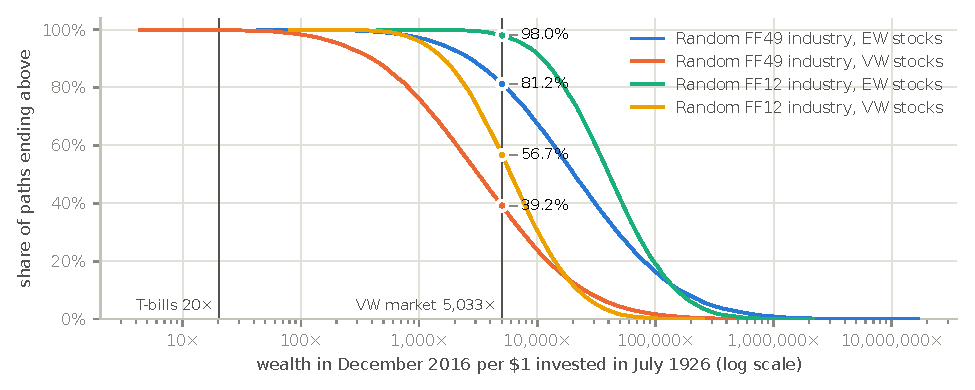
\includegraphics[width=\textwidth]{fig_random_industry.pdf}
  \caption{Full-period wealth of the 20,000 random-industry paths. Each curve gives the share of paths ending
    above a given wealth level. Dots mark the share that beat the VW market.}
  \label{fig:random}
\end{figure}

FF49 EW
    beats the market in 51.7\%, 59.5\% and 81.2\% of outcomes, against at most 49.3\%, 47.5\% and 43.3\% for the
    paper's 100-stock portfolio. It is far from the single stock's 3.97\% over the full period. It also beats
    T-bills in all 20,000 full-period paths, where only 27.5\% of the paper's single stocks did.

FF49
    VW's shares (49.0\%, 46.4\%, 39.2\%) lie inside the paper's 25- to 100-stock range at every horizon. This
    concerns that one statistic, not the whole distribution. Its 1-year skewness is 1.32, against 6.99 for a single
    stock, which is consistent with diversification within industries. The comparison does not isolate that effect,
    however, and the data vintage and construction also differ from the paper's.

Equal weighting within industries raises the share beating the market by 2.7, 13.2 and 42.0 percentage
points at the three horizons, using the same draws. Its exact 1-year mean is 17.1\% against 13.2\% for VW, before the unmeasured costs of
    maintaining equal weights. The broader FF12 industries have higher shares and much less skewness than FF49.


\subsection{Three-month industry momentum}\label{sec:momentum}

Each month $t$ we hold the industry with the highest compounded return over months $t-3$ to $t-1$, among industries
that are eligible in month $t$ and have all three lookback returns. Ties go to the first in column order. Ranking
and holding use the same returns (EW or VW), and the first holding month is October 1926. Momentum is a single
path, so we compare it with the 20,000 random paths of Section~\ref{sec:random} over the same months
(Tables~\ref{tab:momentum} and~\ref{tab:momperf}, Figure~\ref{fig:momentum}). The lookback requirement makes
momentum's candidate set smaller than the random baseline's in 21 FF49 months, just after an industry enters;
restricting the baseline accordingly would raise its exact mean wealth by under 1\%.

\begin{table}[!htbp]
  \centering\tablefont
  \caption{Three-month industry momentum against random industry selection, October 1926 to December 2016. The
    random mean is exact (Eq.~\ref{eq:exact}). The percentile is the share of random paths with lower full-period
    wealth. Window columns give the share of calendar years, paper decades and rolling 10-year windows in which the
    strategy beat the VW market, shown as momentum\,/\,random.}
  \label{tab:momentum}
  \begin{tabular}{@{}lrrrlrrr@{}}
\toprule
& \multicolumn{3}{c}{Wealth per \$1} & Percentile & \multicolumn{3}{c}{\% of windows $>$ VW market} \\
\cmidrule(lr){2-4} \cmidrule(l){6-8}
Variant & Momentum & Random median & Random mean & [95\% CI] & Years & Decades & Rolling 10y \\ \midrule
FF49 EW & 33,320 & 19,430 & 69,258 & 63.16 [62.49, 63.83] & 54.4 / 51.7 & 66.7 / 59.6 & 69.6 / 61.7 \\
FF49 VW & 113 & 2,968 & 10,993 & 2.22 [2.02, 2.43] & 47.8 / 49.0 & 33.3 / 46.4 & 46.5 / 48.3 \\
FF12 EW & 39,337,330 & 38,766 & 65,110 & 100.00 [99.98, 100.00] & 71.1 / 54.5 & 100.0 / 69.7 & 94.6 / 70.8 \\
FF12 VW & 136,822 & 5,574 & 9,237 & 99.94 [99.90, 99.97] & 66.7 / 50.4 & 88.9 / 51.8 & 83.9 / 51.8 \\
\midrule
VW market & 4,715 & & & & & & \\
T-bills & 20 & & & & & & \\
\bottomrule
\end{tabular}

\end{table}

\begin{table}[!htbp]
  \centering\tablefont
  \caption{Performance, October 1926 to December 2016, before costs. Return and volatility are annualized (\%).
    The Sharpe ratio is over T-bills. Turnover is one-way turnover across industry portfolios (\% a year).
    ``Equal weight'' holds every eligible industry equally, which is the expected outcome of random selection.}
  \label{tab:momperf}
  \begin{tabular}{@{}lrrrrlr@{}}
\toprule
Strategy & Wealth & Return & Volatility & Sharpe & Max drawdown (peak to trough) & Turnover \\
\midrule
Momentum, FF49 EW & 33,320 & 12.2 & 35.9 & 0.40 & $-$99.7 (1929-07 to 1942-03) & 761 \\
Momentum, FF49 VW & 113 & 5.4 & 32.9 & 0.23 & $-$99.2 (1929-08 to 1941-04) & 811 \\
Momentum, FF12 EW & 39,337,330 & 21.4 & 26.4 & 0.74 & $-$83.7 (1929-09 to 1932-05) & 574 \\
Momentum, FF12 VW & 136,822 & 14.0 & 20.6 & 0.58 & $-$71.1 (1929-09 to 1932-05) & 677 \\
\midrule
Equal weight, FF49 EW & 69,258 & 13.1 & 24.9 & 0.48 & $-$85.0 (1929-08 to 1932-05) & 19 \\
Equal weight, FF49 VW & 10,993 & 10.9 & 20.7 & 0.44 & $-$85.3 (1929-08 to 1932-06) & 20 \\
Equal weight, FF12 EW & 65,110 & 13.1 & 24.0 & 0.49 & $-$84.7 (1929-08 to 1932-05) & 13 \\
Equal weight, FF12 VW & 9,237 & 10.6 & 18.5 & 0.46 & $-$83.4 (1929-08 to 1932-05) & 13 \\
\midrule
VW market & 4,715 & 9.8 & 18.6 & 0.42 & $-$83.7 (1929-08 to 1932-06) & -- \\
T-bills & 20.14 & 3.4 & 0.9 & -- & $-$0.1 (1938-10 to 1941-04) & -- \\
\bottomrule
\end{tabular}

\end{table}

\begin{figure}[!htbp]
  \centering
  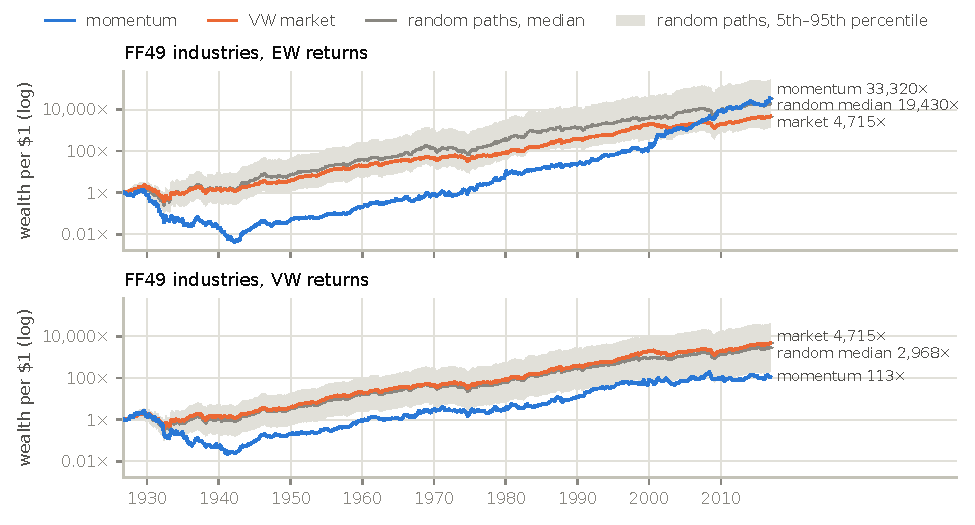
\includegraphics[width=\textwidth]{fig_momentum.pdf}
  \caption{Wealth of FF49 three-month momentum, the VW market and the random-industry paths (median and 5th--95th
    percentile band), October 1926 to December 2016.}
  \label{fig:momentum}
\end{figure}

FF49 EW momentum grew \$1 to 33,320$\times$, against 4,715$\times$ for the market and 19,430$\times$ for the median
    random path, which places it at the 63rd percentile. It fell short of the 69,258$\times$ expected wealth of random
    selection (Eq.~\ref{eq:exact}). It beat the market in 54.4\% of years, 6 of 9 decades and 69.6\% of rolling
    10-year windows.

Wealth fell 99.7\% from 1929 to 1942, and volatility was 35.9\%. The Sharpe
    ratio of 0.40 is below the market's 0.42 and the equal-weight portfolio's 0.48. Momentum held an industry with at
    most five firms in 34\% of months, against 15\% under random selection, and its most frequent holdings were Gold,
    Coal and Smoke. A plausible but untested mechanism is that ranking on noisy three-month returns favors the most
    volatile industries, which in FF49 often have few firms.

FF49 VW momentum ended at 113$\times$ (2nd
    percentile). EW and VW momentum rank on different returns and hold different industries in 696 of 1,083 months,
    so this gap reflects both rankings and holding returns, not weighting alone. With the broad FF12 industries,
    momentum beat every random path with EW returns (Sharpe 0.74) and 99.9\% of them with VW returns. Turnover is
    574\%--811\% a year, so trading costs would matter.


\subsection{Bonus: diversified industry momentum}

For the bonus, we compare two ways of diversifying across industries. Both rebalance monthly and use
value-weighted stock returns within each industry. We assess how often they beat the market over ten years.
\begin{itemize}
  \item \textbf{(a) Equal weight:} hold every eligible FF49 industry equally, value-weighted within each industry,
    rebalanced monthly. This is the expected outcome of random FF49 VW selection.
  \item \textbf{(b) Top 5, 6-month momentum:} each month, hold the five FF49 industries with the highest return over
    months $t-6$ to $t-1$ (Moskowitz and Grinblatt's industry momentum), equally weighted and value-weighted within
    each industry. Holding five industries rather than one diversifies away the single-industry risk documented in
    Section~\ref{sec:momentum}, and value weighting limits the influence of tiny firms.
\end{itemize}
The rules are evaluated from January 1927 to August 2026. We ask whether each rule beats the VW
market in at least 50\% of the paper's nine decades \emph{and} of the 249 rolling 10-year windows that lie entirely
within January 1996 to August 2026. Because Sections~\ref{sec:random} and~\ref{sec:momentum} use data through 2016,
this holdout is a retrospective validation. Adjacent rolling windows share 119 months, and the holdout contains only
three non-overlapping decades, so its 249 windows are not independent confirmations. January 2017 to August 2026
(116 months, with no complete 10-year window) lies outside the earlier samples. It is reported separately as a
post-2016 evaluation of the candidates. It is not an independent test of the final choice: those months
also enter the screen and the comparison between the two rules.

\begin{table}[!htbp]
  \centering\tablefont
  \caption{Win rates against the VW market over 10-year windows (strictly higher holding return), before costs.
    The two rows marked ``screen'' form the pass/fail criterion.}
  \label{tab:screen}
  \begin{tabular}{@{}lrrrrr@{}}
\toprule
& & \multicolumn{2}{c}{(a) equal weight} & \multicolumn{2}{c}{(b) top 5, 6-month} \\
\cmidrule(lr){3-4} \cmidrule(l){5-6}
Measure & Windows & Wins & Win rate & Wins & Win rate \\ \midrule
Paper decades to 2016 \textbf{(screen)} & 9 & 7 & 77.8\% & 8 & 88.9\% \\
Holdout rolling 10-year windows \textbf{(screen)} & 249 & 154 & 61.8\% & 206 & 82.7\% \\
\midrule
Pre-1996: paper decades ending by Dec 1986 & 6 & 5 & 83.3\% & 6 & 100.0\% \\
Pre-1996: rolling windows ending by Dec 1995 & 709 & 549 & 77.4\% & 569 & 80.3\% \\
Holdout decades 1996--2005, 2006--2015, 2016--2025 & 3 & 2 & 66.7\% & 3 & 100.0\% \\
All rolling 10-year windows & 1,077 & 748 & 69.5\% & 845 & 78.5\% \\
\bottomrule
\end{tabular}

\end{table}

\begin{table}[!htbp]
  \centering\tablefont
  \caption{Performance by period, before costs. Wealth is per \$1. Return and volatility are annualized (\%).
    Turnover is one-way across industries (\% a year). Jan 2017--Aug 2026 is the post-2016 evaluation period (116 months).}
  \label{tab:ruleperf}
  \begin{tabular}{@{}llrrrrrr@{}}
\toprule
Period & Strategy & Wealth & Return & Volatility & Sharpe & Max drawdown & Turnover \\ \midrule
Jan 1927--Aug 2026 & (a) equal weight & 35,774 & 11.1 & 20.3 & 0.46 & $-$85.3 & 20 \\
 & (b) top 5 & 662,986 & 14.4 & 22.0 & 0.58 & $-$82.6 & 455 \\
 & VW market & 17,985 & 10.3 & 18.4 & 0.45 & $-$83.7 & -- \\
\addlinespace
Jan 1927--Dec 1995 & (a) equal weight & 1,458 & 11.1 & 21.9 & 0.42 & $-$85.3 & 20 \\
 & (b) top 5 & 9,548 & 14.2 & 22.6 & 0.54 & $-$82.6 & 446 \\
 & VW market & 816 & 10.2 & 19.4 & 0.41 & $-$83.7 & -- \\
\addlinespace
Jan 1996--Aug 2026 & (a) equal weight & 24.53 & 11.0 & 16.4 & 0.58 & $-$52.6 & 21 \\
 & (b) top 5 & 69.44 & 14.8 & 20.5 & 0.67 & $-$50.4 & 476 \\
 & VW market & 22.04 & 10.6 & 15.7 & 0.58 & $-$50.3 & -- \\
\addlinespace
Jan 2017--Aug 2026 & (a) equal weight & 3.32 & 13.2 & 17.1 & 0.68 & $-$25.9 & 21 \\
 & (b) top 5 & 4.61 & 17.1 & 22.2 & 0.72 & $-$23.1 & 471 \\
 & VW market & 3.92 & 15.2 & 16.1 & 0.81 & $-$24.8 & -- \\
\bottomrule
\end{tabular}

\end{table}

\begin{figure}[!htbp]
  \centering
  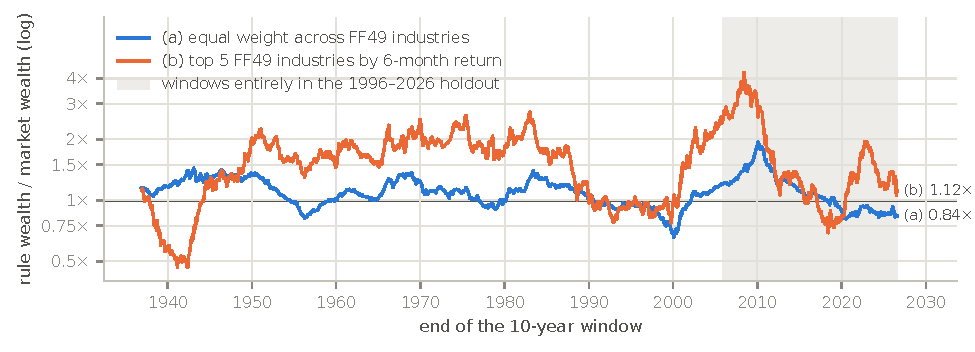
\includegraphics[width=\textwidth]{fig_rules.pdf}
  \caption{Each rule's rolling 10-year wealth relative to the VW market, at the window's end; above 1$\times$, the
    rule won.}
  \label{fig:rules}
\end{figure}

We favor the top-five momentum rule. It beats the market in 8 of the paper's 9 decades, 206 of 249
later-period rolling windows, and 845 of all 1,077 rolling ten-year windows since 1927 (78.5\%). Over the
full sample, it returns 14.4\% a year against the market's 10.3\%, with a Sharpe ratio of 0.58 against 0.45.
It also wins over January 2017--August 2026 (4.61$\times$ versus 3.92$\times$), although its Sharpe ratio
is lower in that period (0.72 versus 0.81).

The equally weighted industry portfolio has lost every rolling window ending since March 2019. The
momentum rule has the stronger historical record, but its 78.5\% win rate comes from overlapping windows
used in the same strategy comparison. It is not an established probability of beating the market over
the next decade. Annual turnover is about 455\%, roughly 23 times the equal-weight rule's, so trading
costs would reduce the reported advantage.

%======================================================================================================
\section{Limitations}
All results are before transaction costs, and turnover counts trades between industries only. The returns come from
the current, revised CRSP data (CIZ format), not the FIZ-era data the paper used, and the size of that difference is
not measured. Industries are not stocks, and FF12 is not a GICS sector scheme. Pooling across windows and dropping
the partial year 1926 are our choices; the paper documents neither. The industry simulations use a single seed.

\textbf{Code and data.} All computations are in \nolinkurl{hw2_analysis.ipynb}, using the tested modules in
\nolinkurl{src/}. \nolinkurl{report/make_tables.py} and \nolinkurl{report/make_figures.py} rebuild these tables and
figures from \nolinkurl{output/} and check them against it.

\textbf{References.}
{\footnotesize
Ang, A., R. Hodrick, Y. Xing and X. Zhang (2006), The cross-section of volatility and expected returns,
\emph{Journal of Finance} 61.
Baker, M., B. Bradley and J. Wurgler (2011), Benchmarks as limits to arbitrage: understanding the low-volatility
anomaly, \emph{Financial Analysts Journal} 67.
Bessembinder, H. (2018), Do stocks outperform Treasury bills?, \emph{Journal of Financial Economics} 129.
Frazzini, A. and L. Pedersen (2014), Betting against beta, \emph{Journal of Financial Economics} 111.
Moskowitz, T. and M. Grinblatt (1999), Do industries explain momentum?, \emph{Journal of Finance} 54.
}

\end{document}
